\documentclass[12pt,a4paper]{article}
\usepackage{geometry}
\geometry{margin=1in}
\usepackage{setspace}
\usepackage{amsmath}
\usepackage{graphicx}
\usepackage{enumitem}
\usepackage{titlesec}
\usepackage{titling}
\usepackage{tikz} % TikZ is the base drawing library
\usepackage[siunitx, american]{circuitikz} % circuitikz handles the electrical symbols and units

\setstretch{1.3}

\begin{document}

\begin{center}
    \Large \textbf{PT 100} \\[10pt]
    \normalsize
    \textbf{EE25BTECH11019 - Vivek} \\
    \textbf{EE25BTECH11001 - Aarush}
\end{center}

\vspace{1cm}

\noindent \textbf{Aim:} To measure and analyse the voltage output of PT-100 at varying temperature. \\[10pt]

\noindent \textbf{Components required:}
\begin{enumerate}[label=\arabic*.]
    \item Breadboard
    \item Arduino
    \item PT-100 Sensor
    \item Resistor
    \item Jumper cables
    \item Electric kettle
    \item Thermometer
    \item Mobile with PlatformIO
\end{enumerate}

\vspace{8pt}

\noindent \textbf{Theory:} \\
PT-100 is a platinum resistance temperature detector (RTD). The resistance of platinum changes with temperature. ``PT'' stands for platinum and ``100'' for it having a resistance of $100\,\Omega$ at $0^\circ C$.

\vspace{10pt}

\noindent \textbf{Procedure:}\\[4pt]
\textbf{Connections:}
\begin{enumerate}[label=\arabic*.]
    \item Arrange all circuit components as shown in the figure behind the page.
    \item Electric kettle is used to increase the temperature of PT-100, and values are measured using the next step.
\end{enumerate}
\newpage
\noindent \textbf{Circuit Diagram(without LCD)} \\

\begin{figure}[h!]
 \centering
 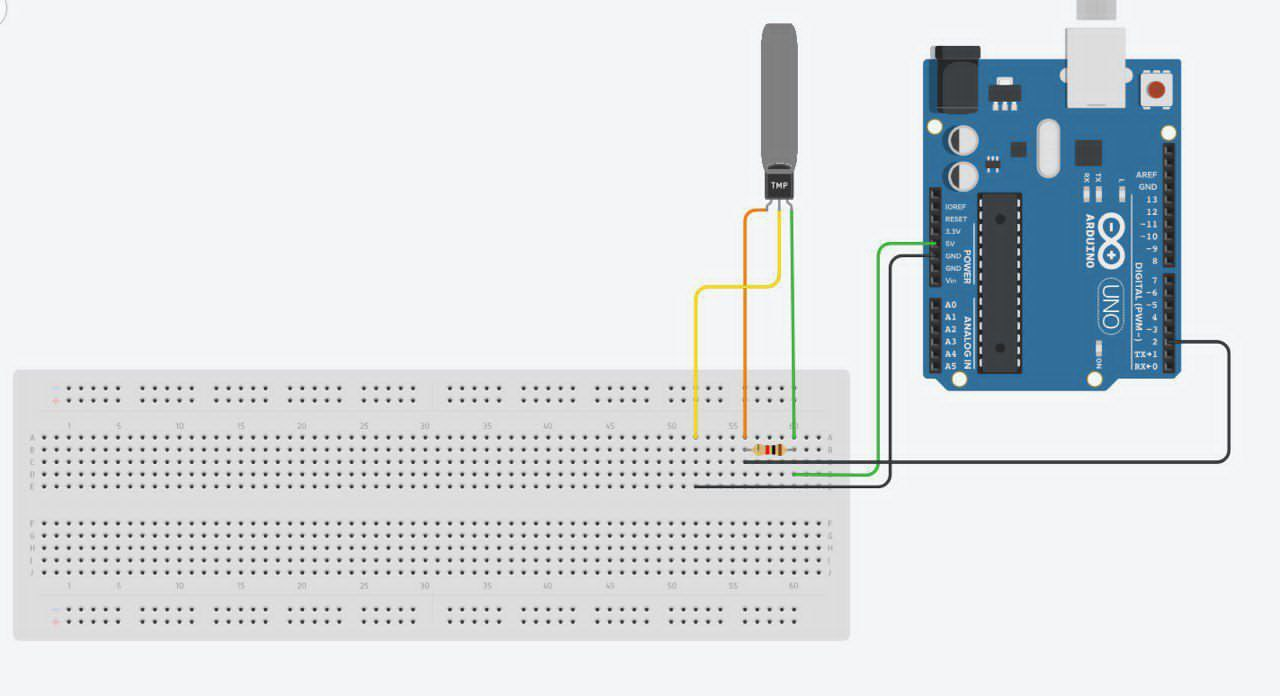
\includegraphics[width=0.75\columnwidth]{arduino.jpg}
\end{figure}

\begin{figure}[h!]
    \centering
    \begin{circuitikz}[american, scale=1.2]
        % Battery
        \draw
        (0,0) to[battery1, l_=5V] (0,3)
        % 150 ohm resistor
        to[R=150$\Omega$] (3,3)
        % Node a
        node[circ, label=right:$a$] (a) {}
        % PT100 resistor to ground
        (a) to[R=$  P\,\Omega$ (PT-100 Resistance)] (3,0)
        % Connect back to ground
        -- (0,0);
        
        % Label for ground node
        \node at (3.2,-0.2) {o};
    \end{circuitikz}
\end{figure}

\newpage

\section*{4. Observations : (Training Data)}

\begin{table}[h!]
\centering
\begin{tabular}{|c|c|}
\hline
\textbf{Temperature ($^\circ$C)} & \textbf{Voltage (V)} \\ \hline
26.1 & 2.1603 \\ 
27.9 & 2.1652 \\ 
32.6 & 2.1847 \\ 
34.4 & 2.1896 \\ 
36.5 & 2.1994 \\ 
38.4 & 2.2092 \\ 
42.8 & 2.2238 \\ 
45.3 & 2.2336 \\ 
48.9 & 2.2483 \\ 
52.1 & 2.2629 \\ 
53.8 & 2.2678 \\ 
56.7 & 2.2776 \\ 
60.6 & 2.2923 \\ 
61.7 & 2.2971 \\ 
63.6 & 2.3069 \\ 
65.8 & 2.3118 \\ 
68.5 & 2.3216 \\ 
69.3 & 2.3265 \\ 
71.9 & 2.3362 \\ 
78.5 & 2.3607 \\ 
89.8 & 2.3998 \\ \hline
\end{tabular}
\end{table}

\begin{figure}[h!]
    \centering
    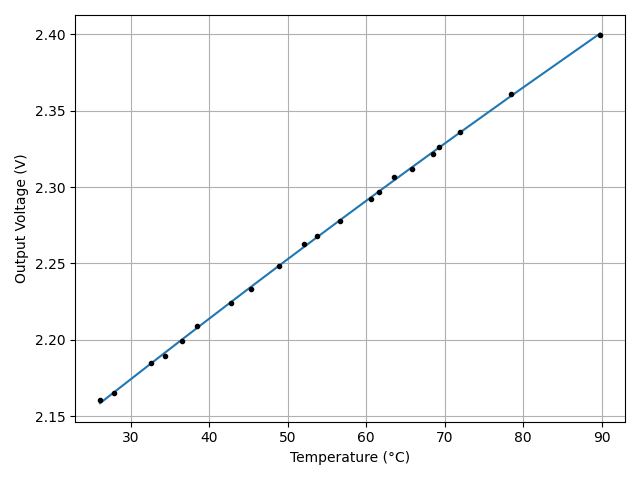
\includegraphics[width=0.8\textwidth]{../figs/train.png}
\end{figure}

\newpage

\section*{5. Observations : (Validation Data)}

\begin{table}[h!]
\centering
\begin{tabular}{|c|c|}
\hline
\textbf{Temperature ($^\circ$C)} & \textbf{Voltage (V)} \\ \hline
29.8 & 2.1749 \\ 
35.1 & 2.1945 \\ 
40.5 & 2.2141 \\ 
47.0 & 2.2434 \\ 
50.3 & 2.2532 \\ 
57.0 & 2.2825 \\ 
62.7 & 2.3020 \\ 
66.8 & 2.3167 \\ 
70.2 & 2.3318 \\ 
73.8 & 2.3411 \\ 
85.5 & 2.3851 \\ 
91.2 & 2.4046 \\ 
92.1 & 2.4095 \\ \hline
\end{tabular}
\end{table}

\begin{figure}[h!]
    \centering
    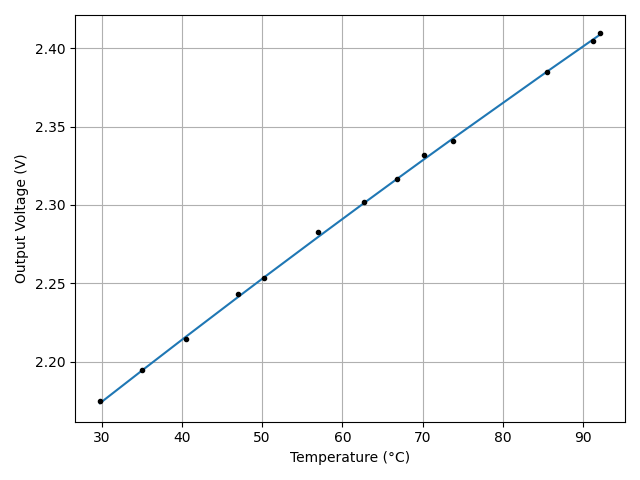
\includegraphics[width=0.8\textwidth]{../figs/valid.png}
\end{figure}

\newpage 

\section*{3. Theory}

Using Callendar–Van Dusen equation,

\[
V(T) = V(0) \begin{pmatrix}1 \\[4pt] A \\[4pt] B \end{pmatrix}
\begin{pmatrix}1 \\[4pt] T \\[4pt] T^2 \end{pmatrix}
\]

\[
\Rightarrow \; C = n^{T}x \quad \text{where } C = V(T), \;
x = \begin{pmatrix}1 \\[4pt] T \\[4pt] T^2 \end{pmatrix}, \;
n = V(0)\begin{pmatrix}1 \\[4pt] A \\[4pt] B \end{pmatrix}
\]

For multiple points,

\[
X^{T}n = C
\]

\[
X =
\begin{pmatrix}
1 & 1 & 1 & \cdots & 1\\
T_1 & T_2 & T_3 & \cdots & T_n\\
T_1^2 & T_2^2 & T_3^2 & \cdots & T_n^2
\end{pmatrix},
\quad
C =
\begin{pmatrix}
V(T_1)\\[4pt]
V(T_2)\\[4pt]
V(T_3)\\[4pt]
\vdots\\[4pt]
V(T_n)
\end{pmatrix}
\]


We will use the above equation to find \( n \).  
Using the least squares method, we estimate:

\[
n = (X^{T}X)^{-1}X^{T}C
\]

\vspace{1em}
\noindent
\section*{Codes:}

The codes for this project may be found at the given URL:  
\begin{center}
	\texttt{https://github.com/spideyboo/Digital-Thermometer}
\end{center}

\noindent
Above codes should be typed in \textbf{PlatformIO} and the mobile should be connected to \textbf{Arduino UNO} so that the codes are compiled and executed.  
These codes are written in \textbf{Embedded C} and the \textbf{ML and Error Analysis (Python)}.

\newpage

\section*{5. Error Analysis}

The quadratic loss function of a linear regression model is defined as

\[
\text{MSE} = \frac{\sum{(y_{\text{exp}} - y_{\text{act}})^2}}{n}
\]

where \( n \) = number of readings.

\vspace{10pt}

For Training data set:
\[
\text{MSE} = 1.41598774 \times 10^{-6}
\]

For Validation data set:
\[
\text{MSE} = 2.31182403 \times 10^{-6}
\]

\begin{figure}[h!]
    \centering
    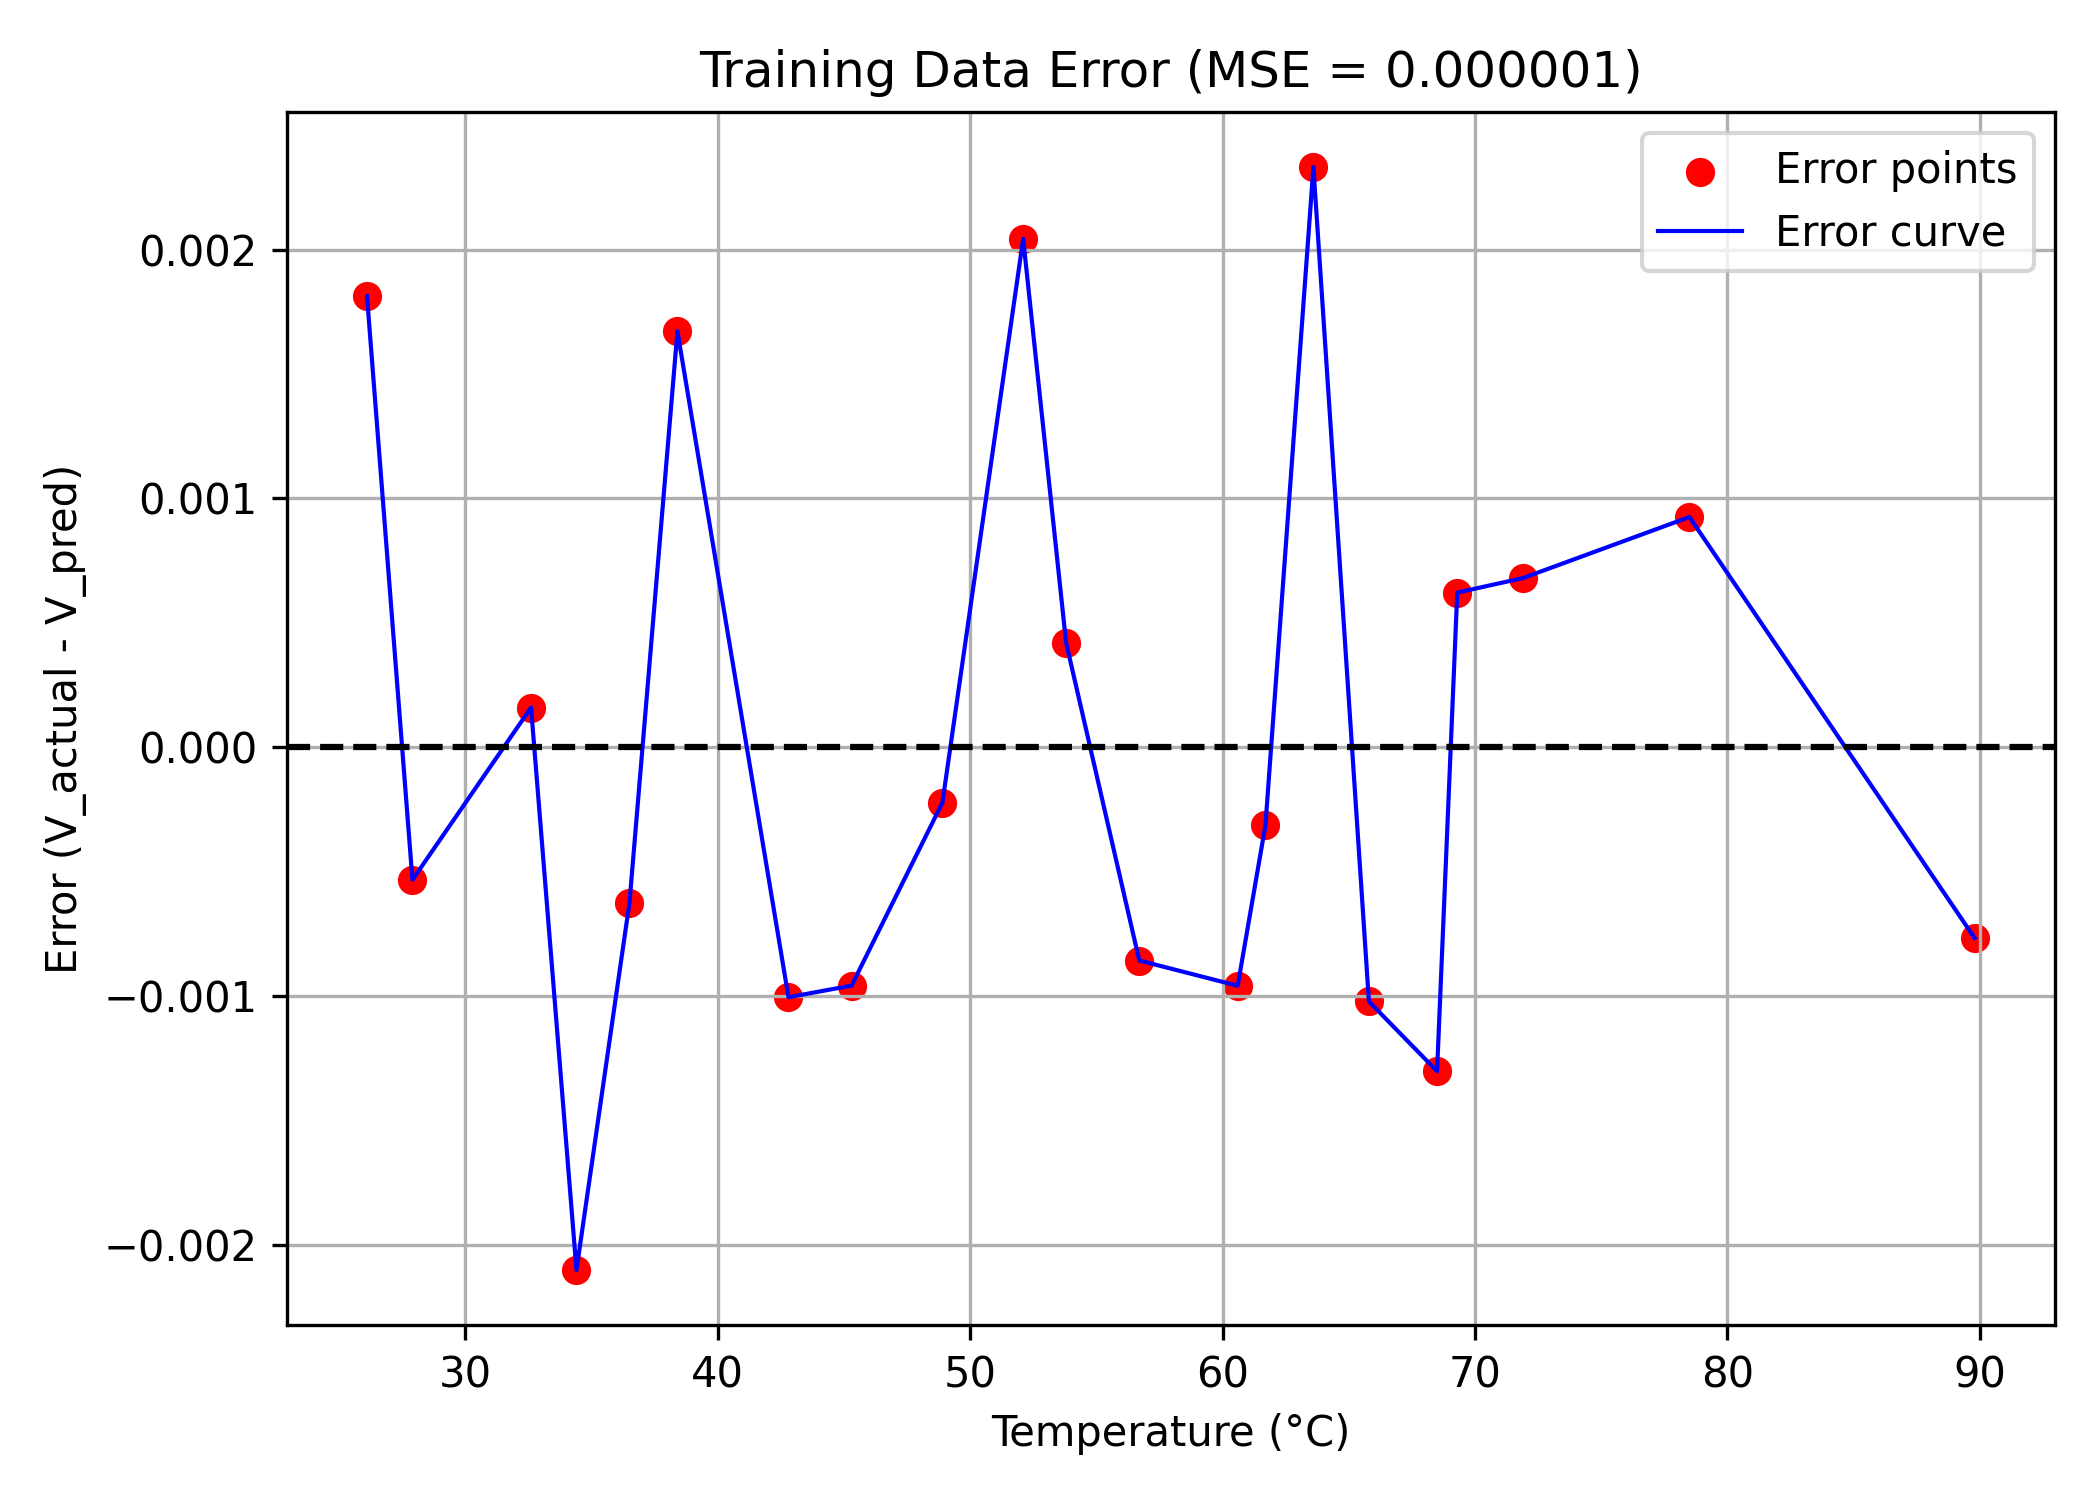
\includegraphics[width=0.85\textwidth]{../figs/train_error.png}
\end{figure}

\begin{figure}[h!]
    \centering
    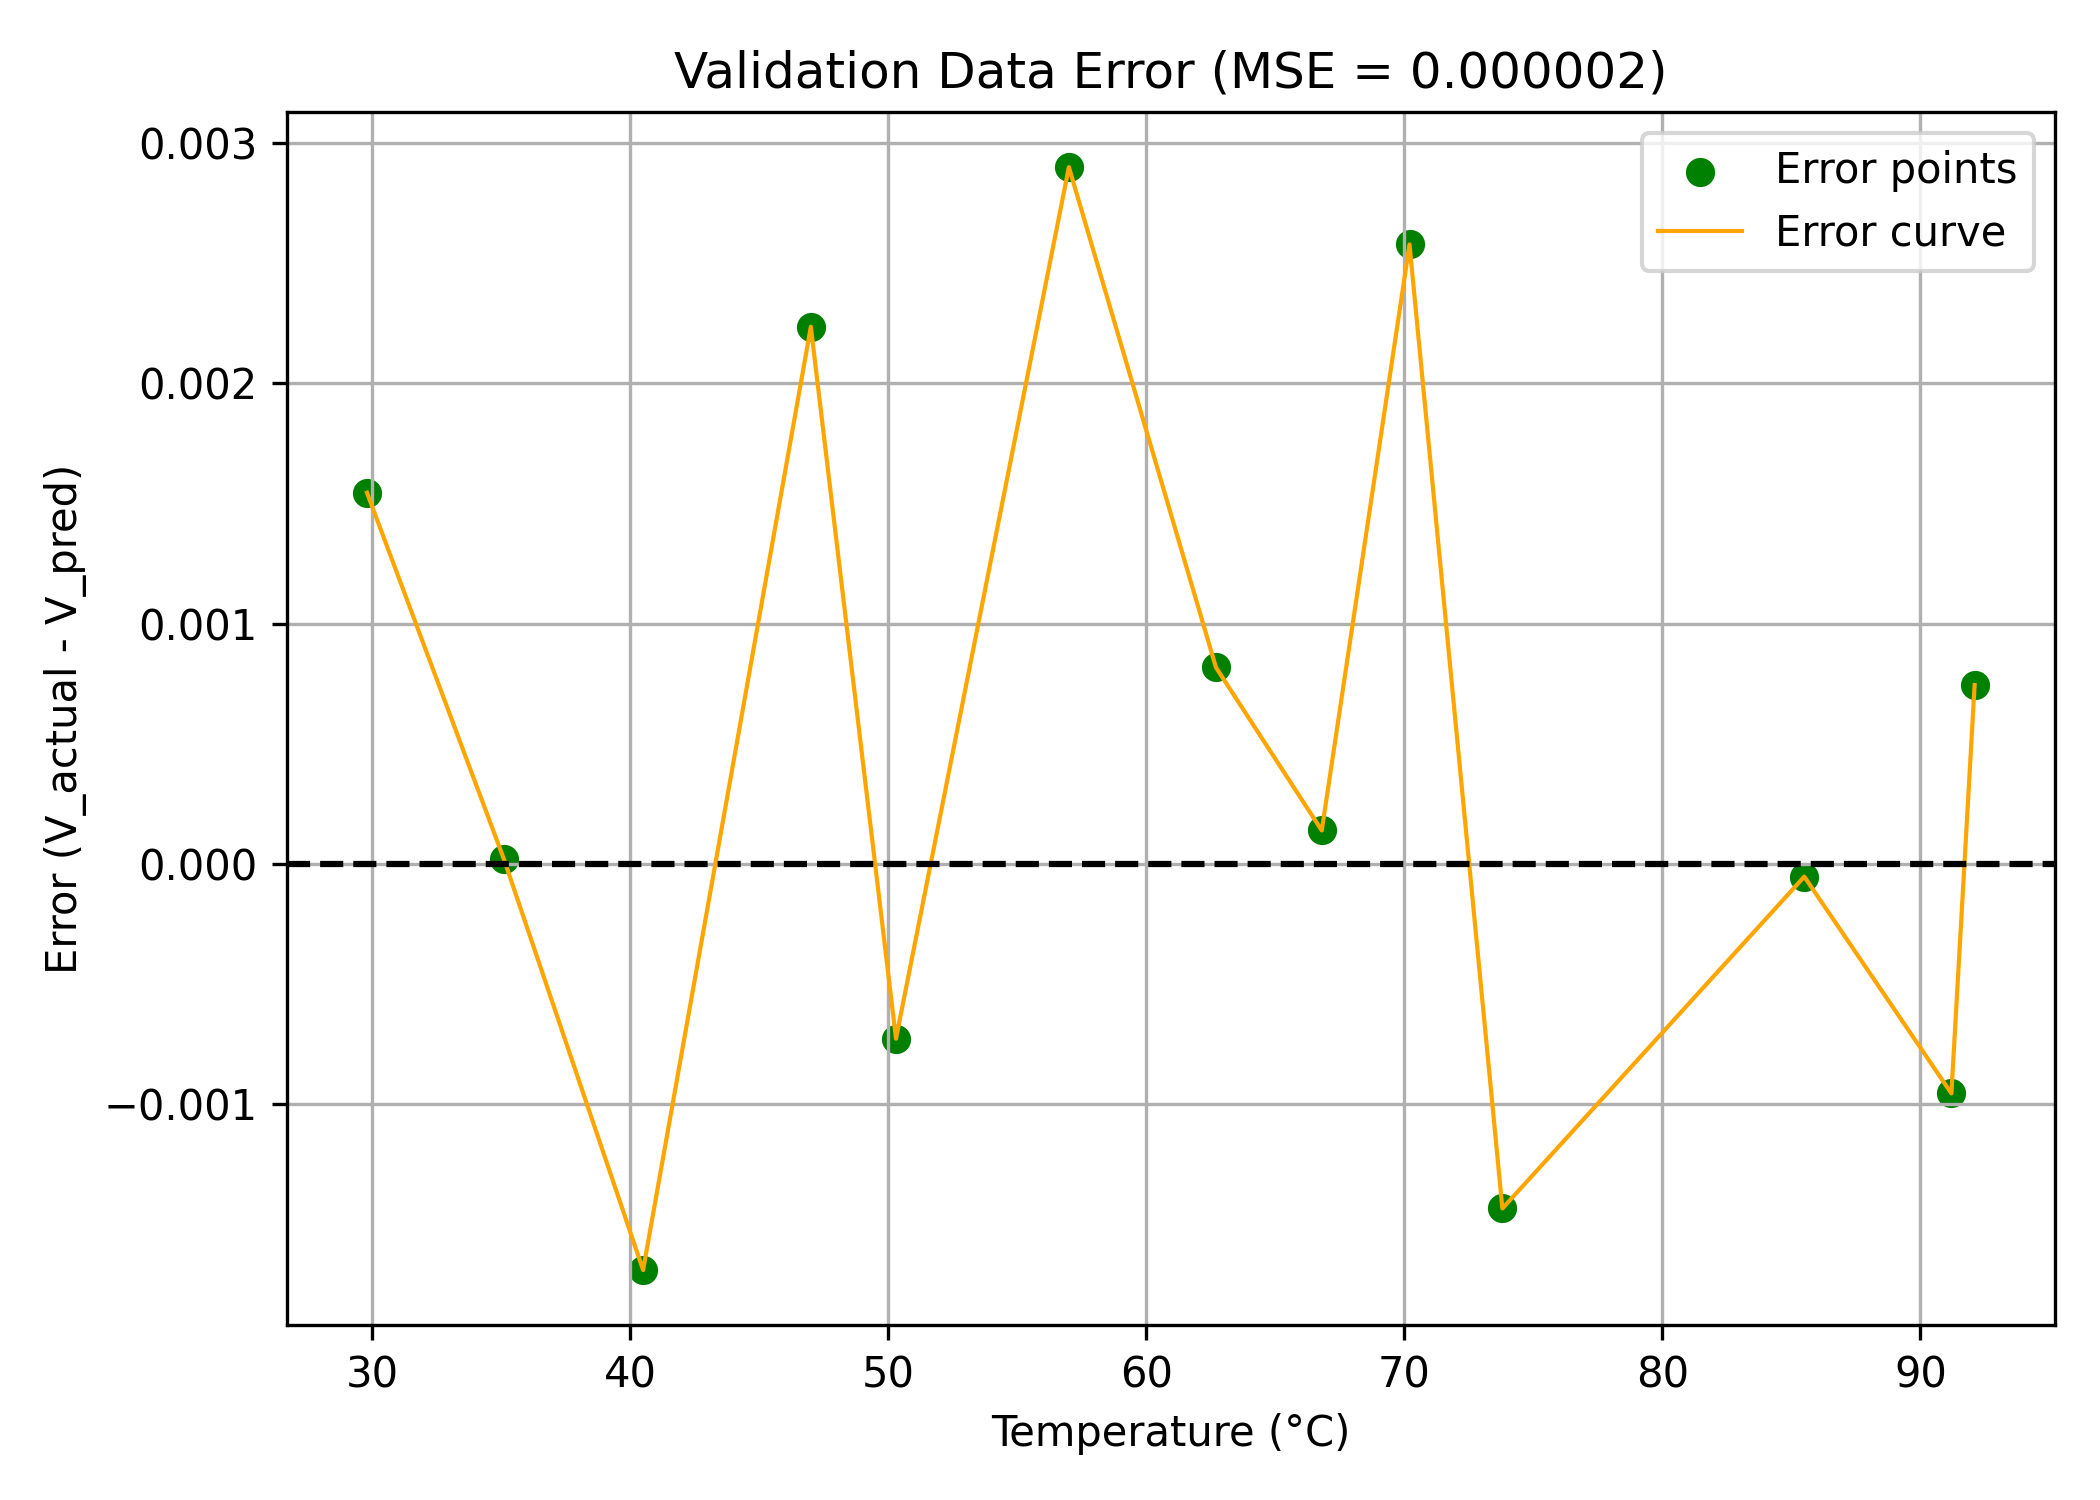
\includegraphics[width=0.85\textwidth]{../figs/valid_error.png}
\end{figure}

\section*{6. Conclusion}

In conclusion, this report successfully demonstrates the use of the PT-100 sensor with Arduino for temperature measurement.  
The project involved setting up a circuit, coding, and data collection to observe the sensor's response across varying temperature.  
The experiment verified the PT-100's effectiveness in providing reliable temperature readings, making it a valuable component for precise temperature monitoring in various applications.


\end{document}
